\documentclass[]{article}
\usepackage{lmodern}
\usepackage{amssymb,amsmath}
\usepackage{ifxetex,ifluatex}
\usepackage{fixltx2e} % provides \textsubscript
\ifnum 0\ifxetex 1\fi\ifluatex 1\fi=0 % if pdftex
  \usepackage[T1]{fontenc}
  \usepackage[utf8]{inputenc}
\else % if luatex or xelatex
  \ifxetex
    \usepackage{mathspec}
  \else
    \usepackage{fontspec}
  \fi
  \defaultfontfeatures{Ligatures=TeX,Scale=MatchLowercase}
\fi
% use upquote if available, for straight quotes in verbatim environments
\IfFileExists{upquote.sty}{\usepackage{upquote}}{}
% use microtype if available
\IfFileExists{microtype.sty}{%
\usepackage{microtype}
\UseMicrotypeSet[protrusion]{basicmath} % disable protrusion for tt fonts
}{}
\usepackage[margin=1in]{geometry}
\usepackage{hyperref}
\hypersetup{unicode=true,
            pdftitle={flgaCBC},
            pdfauthor={Burnett, JL},
            pdfborder={0 0 0},
            breaklinks=true}
\urlstyle{same}  % don't use monospace font for urls
\usepackage{color}
\usepackage{fancyvrb}
\newcommand{\VerbBar}{|}
\newcommand{\VERB}{\Verb[commandchars=\\\{\}]}
\DefineVerbatimEnvironment{Highlighting}{Verbatim}{commandchars=\\\{\}}
% Add ',fontsize=\small' for more characters per line
\usepackage{framed}
\definecolor{shadecolor}{RGB}{248,248,248}
\newenvironment{Shaded}{\begin{snugshade}}{\end{snugshade}}
\newcommand{\AlertTok}[1]{\textcolor[rgb]{0.94,0.16,0.16}{#1}}
\newcommand{\AnnotationTok}[1]{\textcolor[rgb]{0.56,0.35,0.01}{\textbf{\textit{#1}}}}
\newcommand{\AttributeTok}[1]{\textcolor[rgb]{0.77,0.63,0.00}{#1}}
\newcommand{\BaseNTok}[1]{\textcolor[rgb]{0.00,0.00,0.81}{#1}}
\newcommand{\BuiltInTok}[1]{#1}
\newcommand{\CharTok}[1]{\textcolor[rgb]{0.31,0.60,0.02}{#1}}
\newcommand{\CommentTok}[1]{\textcolor[rgb]{0.56,0.35,0.01}{\textit{#1}}}
\newcommand{\CommentVarTok}[1]{\textcolor[rgb]{0.56,0.35,0.01}{\textbf{\textit{#1}}}}
\newcommand{\ConstantTok}[1]{\textcolor[rgb]{0.00,0.00,0.00}{#1}}
\newcommand{\ControlFlowTok}[1]{\textcolor[rgb]{0.13,0.29,0.53}{\textbf{#1}}}
\newcommand{\DataTypeTok}[1]{\textcolor[rgb]{0.13,0.29,0.53}{#1}}
\newcommand{\DecValTok}[1]{\textcolor[rgb]{0.00,0.00,0.81}{#1}}
\newcommand{\DocumentationTok}[1]{\textcolor[rgb]{0.56,0.35,0.01}{\textbf{\textit{#1}}}}
\newcommand{\ErrorTok}[1]{\textcolor[rgb]{0.64,0.00,0.00}{\textbf{#1}}}
\newcommand{\ExtensionTok}[1]{#1}
\newcommand{\FloatTok}[1]{\textcolor[rgb]{0.00,0.00,0.81}{#1}}
\newcommand{\FunctionTok}[1]{\textcolor[rgb]{0.00,0.00,0.00}{#1}}
\newcommand{\ImportTok}[1]{#1}
\newcommand{\InformationTok}[1]{\textcolor[rgb]{0.56,0.35,0.01}{\textbf{\textit{#1}}}}
\newcommand{\KeywordTok}[1]{\textcolor[rgb]{0.13,0.29,0.53}{\textbf{#1}}}
\newcommand{\NormalTok}[1]{#1}
\newcommand{\OperatorTok}[1]{\textcolor[rgb]{0.81,0.36,0.00}{\textbf{#1}}}
\newcommand{\OtherTok}[1]{\textcolor[rgb]{0.56,0.35,0.01}{#1}}
\newcommand{\PreprocessorTok}[1]{\textcolor[rgb]{0.56,0.35,0.01}{\textit{#1}}}
\newcommand{\RegionMarkerTok}[1]{#1}
\newcommand{\SpecialCharTok}[1]{\textcolor[rgb]{0.00,0.00,0.00}{#1}}
\newcommand{\SpecialStringTok}[1]{\textcolor[rgb]{0.31,0.60,0.02}{#1}}
\newcommand{\StringTok}[1]{\textcolor[rgb]{0.31,0.60,0.02}{#1}}
\newcommand{\VariableTok}[1]{\textcolor[rgb]{0.00,0.00,0.00}{#1}}
\newcommand{\VerbatimStringTok}[1]{\textcolor[rgb]{0.31,0.60,0.02}{#1}}
\newcommand{\WarningTok}[1]{\textcolor[rgb]{0.56,0.35,0.01}{\textbf{\textit{#1}}}}
\usepackage{graphicx,grffile}
\makeatletter
\def\maxwidth{\ifdim\Gin@nat@width>\linewidth\linewidth\else\Gin@nat@width\fi}
\def\maxheight{\ifdim\Gin@nat@height>\textheight\textheight\else\Gin@nat@height\fi}
\makeatother
% Scale images if necessary, so that they will not overflow the page
% margins by default, and it is still possible to overwrite the defaults
% using explicit options in \includegraphics[width, height, ...]{}
\setkeys{Gin}{width=\maxwidth,height=\maxheight,keepaspectratio}
\IfFileExists{parskip.sty}{%
\usepackage{parskip}
}{% else
\setlength{\parindent}{0pt}
\setlength{\parskip}{6pt plus 2pt minus 1pt}
}
\setlength{\emergencystretch}{3em}  % prevent overfull lines
\providecommand{\tightlist}{%
  \setlength{\itemsep}{0pt}\setlength{\parskip}{0pt}}
\setcounter{secnumdepth}{0}
% Redefines (sub)paragraphs to behave more like sections
\ifx\paragraph\undefined\else
\let\oldparagraph\paragraph
\renewcommand{\paragraph}[1]{\oldparagraph{#1}\mbox{}}
\fi
\ifx\subparagraph\undefined\else
\let\oldsubparagraph\subparagraph
\renewcommand{\subparagraph}[1]{\oldsubparagraph{#1}\mbox{}}
\fi

%%% Use protect on footnotes to avoid problems with footnotes in titles
\let\rmarkdownfootnote\footnote%
\def\footnote{\protect\rmarkdownfootnote}

%%% Change title format to be more compact
\usepackage{titling}

% Create subtitle command for use in maketitle
\newcommand{\subtitle}[1]{
  \posttitle{
    \begin{center}\large#1\end{center}
    }
}

\setlength{\droptitle}{-2em}

  \title{flgaCBC}
    \pretitle{\vspace{\droptitle}\centering\huge}
  \posttitle{\par}
    \author{Burnett, JL}
    \preauthor{\centering\large\emph}
  \postauthor{\par}
      \predate{\centering\large\emph}
  \postdate{\par}
    \date{February 20, 2019}

\usepackage{booktabs}
\usepackage{longtable}
\usepackage{array}
\usepackage{multirow}
\usepackage{wrapfig}
\usepackage{float}
\usepackage{colortbl}
\usepackage{pdflscape}
\usepackage{tabu}
\usepackage{threeparttable}
\usepackage{threeparttablex}
\usepackage[normalem]{ulem}
\usepackage{makecell}
\usepackage{xcolor}

\begin{document}
\maketitle

\begin{Shaded}
\begin{Highlighting}[]
\CommentTok{## SPECIES TO INCLUDE}
\CommentTok{# You can count hummingbird sp, Archilochus sp., waterthrush sp., Empidonax sp. as Neotropical migrants,   Crow sp. as urban adapters, accipiter sp. as feeder adapters. I'd say ignore the rest.   }
\end{Highlighting}
\end{Shaded}

\hypertarget{flga-cbc}{%
\subsection{FLGA CBC}\label{flga-cbc}}

\begin{figure}
\centering
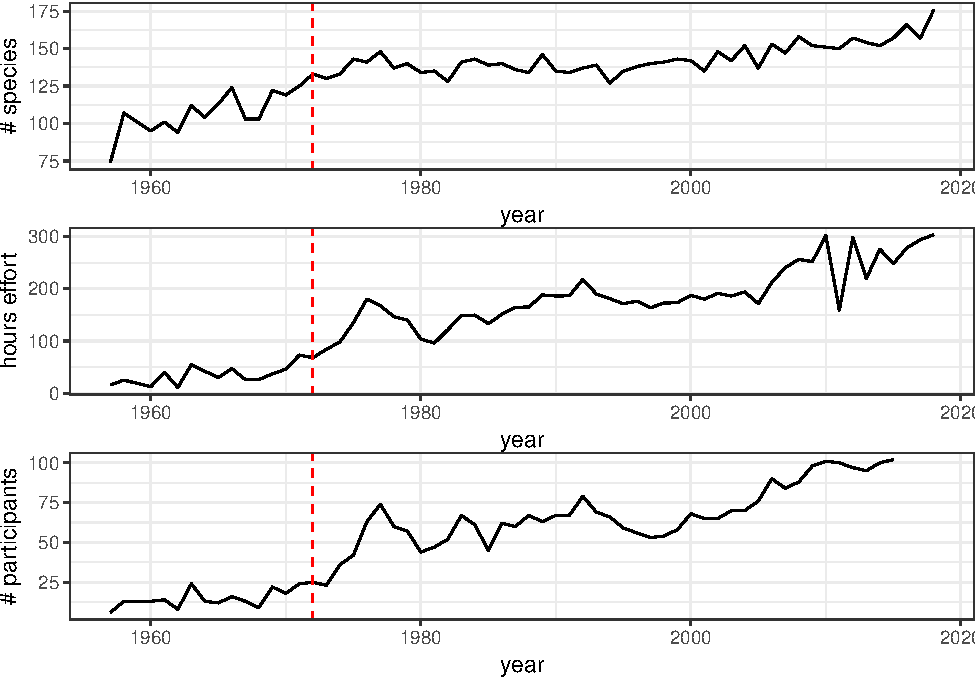
\includegraphics{runThrough_files/figure-latex/effortPlots-1.pdf}
\caption{Annual effort and species richness for the FLGA CBC circle.
Dashed line indicates year we begin analyses.}
\end{figure}

The count format (broken up into 11 teams and all day counts) was
instituted in 1972, so i think that would be a good time to begin.
Therefore, we analze data from 1972 to 2018.

\hypertarget{species-groups}{%
\subsection{Species groups}\label{species-groups}}

\begin{longtable}{llllllllllll}
\caption{\label{tab:sppGroupTab}Species groups for analysis}\\
\toprule
species & Neotropical migrants & Short-distance migrants & Locally endemic & Widespread declining & Non-native & N. FL wintering center & DDT-vics & Sweetwater & Urban adapters & Ag-loss vics & Feeder birds\\
\midrule
American Bittern &  &  &  &  &  &  &  & X &  &  & \\
American Crow &  &  &  &  &  & X &  &  & X &  & X\\
American Goldfinch &  &  &  &  &  & X &  &  &  &  & X\\
American Kestrel &  &  &  &  &  &  &  &  &  & X & \\
American Pipit &  &  &  &  &  &  &  &  &  & X & \\
\addlinespace
American Redstart & X &  &  &  &  &  &  &  &  &  & \\
American Robin &  &  &  &  &  & X &  &  &  &  & \\
American Woodcock &  & X &  &  &  &  &  &  &  &  & \\
Anhinga &  &  &  &  &  &  &  & X &  &  & \\
Ash Throated Flycatcher & X &  &  &  &  &  &  &  &  &  & \\
\addlinespace
Bachman's Sparrow &  &  & X &  &  &  &  &  &  &  & \\
Bald Eagle &  &  &  &  &  &  & X &  &  &  & \\
Baltimore Oriole & X &  &  &  &  &  &  &  &  &  & X\\
Barn Owl &  &  &  &  &  &  &  &  & X & X & \\
Belted Kingfisher &  &  &  &  &  & X &  &  &  &  & \\
\addlinespace
Black-And-White-Warbler &  &  &  &  &  & X &  &  &  &  & \\
Black-And-White Warbler & X &  &  &  &  &  &  &  &  &  & \\
Black-Bellied Whistling-Duck &  &  &  &  & X &  &  &  & X &  & \\
Black-Chinned Hummingbird & X &  &  &  &  &  &  &  &  &  & \\
Black-Crowned Night-Heron &  &  &  &  &  &  &  & X &  &  & \\
\addlinespace
Black-Headed Grosbeak & X &  &  &  &  &  &  &  &  &  & \\
Black-Throated Blue Warbler & X &  &  &  &  &  &  &  &  &  & \\
Black Vulture &  &  &  &  &  &  &  &  & X &  & \\
Blue-Gray Gnatcatcher &  &  &  &  &  & X &  &  &  &  & \\
Blue-Headed Vireo &  &  &  &  &  & X &  &  &  &  & \\
\addlinespace
Blue-Winged Teal &  &  &  &  &  &  &  & X &  &  & \\
Blue Jay &  &  &  &  &  & X &  &  & X &  & X\\
Boat-Tailed Grackle &  &  &  &  &  &  &  &  & X & X & \\
Brown-Headed Cowbird &  &  &  &  &  & X &  &  & X &  & X\\
Brown-Headed Nuthatch &  &  & X &  &  &  &  &  &  &  & \\
\addlinespace
Brown Creeper &  & X &  &  &  &  &  &  &  &  & \\
Brown Thrasher &  &  &  & X &  & X &  &  & X & X & \\
Canada Goose &  &  &  &  &  &  &  &  & X &  & \\
Cape May Warbler & X &  &  &  &  &  &  &  &  &  & \\
Carolina Chickadee &  &  &  &  &  & X &  &  & X &  & X\\
\addlinespace
Carolina Wren &  &  &  &  &  & X &  &  & X &  & X\\
Chestnut-Sided Warbler & X &  &  &  &  &  &  &  &  &  & \\
Chipping Sparrow &  &  &  &  &  & X &  &  &  &  & X\\
Common Grackle &  & X &  &  &  &  &  &  & X & X & \\
Common Ground-Dove &  &  &  & X &  &  &  &  &  & X & \\
\addlinespace
Common Yellowthroat &  &  &  &  &  & X &  &  &  &  & \\
Cooper's Hawk &  &  &  &  &  &  & X &  &  &  & X\\
Dark-Eyed Junco &  & X &  &  &  &  &  &  &  &  & \\
Dickcissel & X &  &  &  &  &  &  &  &  &  & \\
Double-Crested Cormorant &  &  &  &  &  &  & X & X &  &  & \\
\addlinespace
Downy Woodpecker &  &  &  &  &  & X &  &  &  &  & \\
Eastern Bluebird &  &  &  &  &  & X &  &  &  & X & \\
Eastern Meadowlark &  &  &  & X &  &  &  &  &  & X & \\
Eastern Phoebe &  &  &  &  &  & X &  &  &  & X & \\
Eastern Screech-Owl &  &  &  &  &  &  &  &  & X &  & \\
\addlinespace
Eastern Towhee &  & X &  &  &  &  &  &  &  &  & \\
Eastern Whip-Poor-Will & X &  &  &  &  &  &  &  &  &  & \\
Eurasian Collared-Dove &  &  &  &  & X &  &  &  & X &  & \\
European Starling &  &  &  &  & X &  &  &  & X &  & \\
Field Sparrow &  &  &  & X &  &  &  &  &  & X & \\
\addlinespace
Fish Crow &  &  &  &  &  & X &  &  & X &  & \\
Fox Sparrow &  & X &  &  &  &  &  &  &  &  & \\
Glossy Ibis &  &  &  &  &  &  &  & X &  &  & \\
Golden-Crowned Kinglet &  & X &  &  &  &  &  &  &  &  & \\
Grasshopper Sparrow &  &  &  & X &  &  &  &  &  &  & \\
\addlinespace
Gray Catbird &  &  &  &  &  & X &  &  &  &  & \\
Great-Crested Flycatcher & X &  &  &  &  &  &  &  &  &  & \\
Great-Horned Owl &  &  &  &  &  &  &  &  & X &  & \\
Great Blue Heron &  &  &  &  &  &  &  & X &  &  & \\
Green Heron &  &  &  &  &  &  &  & X &  &  & \\
\addlinespace
Henslow's Sparrow &  &  &  & X &  &  &  &  &  &  & \\
Hermit Thrush &  & X &  &  &  &  &  &  &  &  & \\
Hooded Merganser &  &  &  &  &  &  &  &  & X &  & \\
Hooded Warbler & X &  &  &  &  &  &  &  &  &  & \\
House Finch &  &  &  &  &  &  &  &  & X &  & X\\
\addlinespace
House Sparrow &  &  &  &  & X &  &  &  & X & X & X\\
House Wren &  &  &  &  &  & X &  &  & X &  & \\
Indigo Bunting & X &  &  &  &  &  &  &  &  &  & X\\
Kentucky Warbler & X &  &  &  &  &  &  &  &  &  & \\
Killdeer &  &  &  &  &  & X &  &  &  & X & \\
\addlinespace
King Rail &  &  &  &  &  &  &  & X &  &  & \\
Least Bittern &  &  &  &  &  &  &  & X &  &  & \\
Limpkin &  &  &  &  &  &  &  & X &  &  & \\
Little Blue Heron &  &  &  &  &  &  &  & X &  &  & \\
Loggerhead Shrike &  &  &  & X &  &  &  &  &  & X & \\
\addlinespace
Louisiana Waterthrush & X &  &  &  &  &  &  &  &  &  & \\
Magnolia Warbler & X &  &  &  &  &  &  &  &  &  & \\
Mallard &  &  &  &  & X &  &  &  & X &  & \\
Mallard-Feral &  &  &  &  & X &  &  &  & X &  & \\
Marsh Wren &  &  &  &  &  &  &  & X &  &  & \\
\addlinespace
Merlin &  &  &  &  &  &  & X &  &  &  & \\
Mourning Dove &  &  &  &  &  & X &  &  &  & X & X\\
Nashville Warbler & X &  &  &  &  &  &  &  &  &  & \\
Northern Bobwhite &  &  &  & X &  &  &  &  &  &  & \\
Northern Cardinal &  &  &  &  &  & X &  &  & X &  & X\\
\addlinespace
Northern Harrier &  & X &  &  &  &  &  &  &  & X & \\
Northern Mockingbird &  &  &  &  &  &  &  &  & X & X & \\
Northern MockingBird &  &  &  &  &  & X &  &  &  &  & \\
Northern Parula & X &  &  &  &  &  &  &  &  &  & \\
Northern Waterthrush & X &  &  &  &  &  &  &  &  &  & \\
\addlinespace
Orange-Crowned Warbler &  &  &  &  &  & X &  &  &  &  & \\
Osprey &  &  &  &  &  &  & X &  &  &  & \\
Ovenbird & X &  &  &  &  &  &  &  &  &  & \\
Painted Bunting & X &  &  &  &  &  &  &  &  &  & X\\
Palm Warbler &  &  &  &  &  & X &  &  &  &  & \\
\addlinespace
Peregrine Falcon &  &  &  &  &  &  & X &  &  &  & \\
Pileated Woodpecker &  &  &  &  &  &  &  &  & X &  & \\
Pine Siskin &  & X &  &  &  &  &  &  &  &  & X\\
Pine Warbler &  &  &  &  &  & X &  &  &  &  & \\
Prairie Warbler & X &  &  &  &  &  &  &  &  &  & \\
\addlinespace
Purple Finch &  & X &  &  &  &  &  &  &  &  & \\
Purple Gallinule &  &  &  &  &  &  &  & X &  &  & \\
Red-Bellied Woodpecker &  &  &  &  &  & X &  &  &  &  & X\\
Red-Breasted Nuthatch &  & X &  &  &  &  &  &  &  &  & X\\
Red-Cockaded Woodpecker &  &  & X &  &  &  &  &  &  &  & \\
\addlinespace
Red-Headed Woodpecker &  &  &  & X &  &  &  &  &  &  & \\
Red-Shouldered Hawk &  &  &  &  &  &  & X &  & X &  & \\
Red-Tailed Hawk &  &  &  &  &  &  &  &  &  & X & \\
Red-Winged Blackbird &  & X &  &  &  &  &  &  &  & X & \\
Ring-Billed Gull &  &  &  &  &  &  &  &  & X &  & X\\
\addlinespace
Rock Dove &  &  &  &  & X &  &  &  & X &  & \\
Rose-Breasted Grosbeak & X &  &  &  &  &  &  &  &  &  & \\
Ruby-Throated Hummingbird & X &  &  &  &  &  &  &  &  &  & \\
Ruby Crowned Kinglet &  &  &  &  &  & X &  &  &  &  & \\
Rufous Hummingbird & X &  &  &  &  &  &  &  &  &  & \\
\addlinespace
Rusty Blackbird &  & X &  &  &  &  &  &  &  &  & \\
Sandhill Crane &  & X &  &  &  &  &  &  &  &  & \\
Sedge Wren &  &  &  &  &  & X &  &  &  &  & \\
Sharp-Shinned Hawk &  & X &  &  &  &  & X &  &  &  & X\\
Snail Kite &  &  &  &  &  &  &  & X &  &  & \\
\addlinespace
Song Sparrow &  & X &  &  &  &  &  &  &  &  & \\
Sora &  &  &  &  &  &  &  & X &  &  & \\
Summer Tanager & X &  &  &  &  &  &  &  &  &  & \\
Swamp Sparrow &  &  &  &  &  & X &  &  &  &  & \\
Tricolored Heron &  &  &  &  &  &  &  & X &  &  & \\
\addlinespace
Tufted Titmouse &  &  &  &  &  & X &  &  & X &  & X\\
Turkey Vulture &  &  &  &  &  &  &  &  & X &  & \\
Vaux's Swift & X &  &  &  &  &  &  &  &  &  & \\
Vermilion Flycatcher & X &  &  &  &  &  &  &  &  &  & \\
Vesper Sparrow &  & X &  &  &  &  &  &  &  & X & \\
\addlinespace
Virginia Rail &  &  &  &  &  &  &  & X &  &  & \\
Western Tanager & X &  &  &  &  &  &  &  &  &  & \\
White-Crowned Sparrow &  & X &  &  &  &  &  &  &  &  & \\
White-Eyed Vireo &  &  &  &  &  & X &  &  &  &  & \\
White-Faced Ibis &  &  &  &  &  &  &  & X &  &  & \\
\addlinespace
White-Throated Sparrow &  & X &  &  &  &  &  &  &  &  & \\
White Ibis &  &  &  &  &  &  &  & X & X &  & \\
Wilson's Warbler & X &  &  &  &  &  &  &  &  &  & \\
Winter Wren &  & X &  &  &  &  &  &  &  &  & \\
Wood Duck &  &  &  &  &  &  &  &  & X &  & \\
\addlinespace
Wood Stork &  &  &  &  &  &  &  & X &  &  & \\
Wood Thrush & X &  &  &  &  &  &  &  &  &  & \\
Worm-Eating Warbler & X &  &  &  &  &  &  &  &  &  & \\
Yellow-Bellied Sapsucker &  &  &  &  &  & X &  &  &  &  & \\
Yellow-Crowned Night-Heron &  &  &  &  &  &  &  & X &  &  & \\
\addlinespace
Yellow-Rumped Warbler &  &  &  &  &  & X &  &  &  &  & \\
Yellow-Throated Vireo & X &  &  &  &  &  &  &  &  &  & \\
Yellow-Throated Warbler &  &  &  &  &  & X &  &  &  &  & X\\
Yellow Breasted Chat & X &  &  &  &  &  &  &  &  &  & \\
\bottomrule
\end{longtable}


\end{document}
